\section{Introduction}
\label{sec:intro}

\begin{figure}[t]
  \centering
  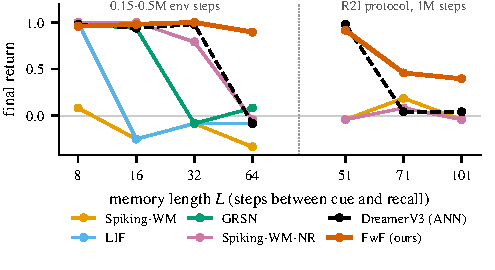
\includegraphics[width=\linewidth]{fig/memory_length}
  \caption{\textbf{Spiking world models forget.}
  Final return on BSuite memory length~\cite{osband2020bsuite}: the agent sees a cue, then $L$ uninformative steps, and is rewarded for recalling the cue (1 = always correct, 0 = chance).
  All models share one spiking world model and differ in the recurrent core (\cref{sec:setup}).
  Left: budgets of 150k to 500k environment steps. Right: $L$ = 51, 71 and 101 with the lengths and budget of R2I~\cite{samsami2024r2i} (1M steps).
  \swm fails at every length, recurrent LIF neurons stop at 8 steps, and GRSN and DH-SNN at 16; TC-LIF, whose state is carried across steps and never cleared, learns 51 and 101 steps \pend{(71: in progress)}.
  \method reaches a return of 0.9 at every length up to 101 steps, and \dv up to 51 (\cref{tab:rl}). \pend{Open markers: runs in progress.}}
  \label{fig:memory_length}
\end{figure}

Spiking neural networks (SNNs)~\cite{maass1997networks} process information with sparse binary spikes, following the dynamics and spike-based communication of biological neurons~\cite{roy2019towards}.
Unlike artificial neural networks (ANNs), spiking neurons trigger synaptic computation only when spikes arrive and replace multiply-accumulate (MAC) operations with accumulate (AC) operations, which take about a fifth of the energy of a MAC on a 45\,nm chip~\cite{horowitz2014energy}; neuromorphic processors exploit this sparsity~\cite{davies2018loihi,orchard2021loihi2}.
Trained directly with surrogate gradients~\cite{neftci2019surrogate,wu2018stbp}, SNNs now classify images with deep residual and transformer architectures~\cite{fang2021sew,zhou2023spikformer,yao2023sdt} and control agents through reinforcement learning (RL)~\cite{tang2020popsan,liu2023dsqn}.
Spiking neurons are also dynamical systems with membrane and dendritic time constants, and these dynamics are widely believed to provide temporal memory~\cite{bellec2018lsnn}.
Neuron models with adaptive thresholds~\cite{bellec2018lsnn,yin2021adaptive}, dendritic branches with heterogeneous time constants~\cite{zheng2024dhsnn}, two compartments~\cite{zhang2024tclif} or gated recurrence~\cite{qin2025grsn} extend this memory on long sequences and in partially observable control.

World models~\cite{ha2018world,hafner2019planet,hafner2020dreamer,hafner2025dreamerv3} compress the history of observations and actions into a recurrent latent state, predict the future from it, and let an agent learn behavior in imagination.
In partially observable environments, this latent state also serves as the agent's memory and must retain information over many steps~\cite{osband2020bsuite,morad2023popgym,pasukonis2023memorymaze}; ANN world models built on state space models retain it for hundreds of steps~\cite{deng2023s4wm,samsami2024r2i}.
A world model updates this state at every step of closed-loop control, so spike-driven computation saves energy at every step, and the dynamics of spiking neurons offer a natural place for its memory.
Accordingly, a recent spiking world model builds on multicompartment neurons whose dendrites integrate over long timescales~\cite{sun2025spikingwm}.

However, existing neuron models and spiking world models extend memory through longer time constants and overlook how the neuron state evolves across environment steps.
Spiking RL methods clear the membrane potentials at the start of every environment step~\cite{tang2020popsan,liu2023dsqn,sun2025spikingwm}, so the time constants act only within a single step.
In the multicompartment neurons of spiking world models, a somatic spike also resets the dendrites~\cite{sun2025spikingwm}, so a dendritic trace survives only until the neuron fires again.
Moreover, the standard Euler update writes input with a gain of $1/\tau$, so compartments with long time constants store their input too weakly to drive spikes.
As a result, existing spiking world models forget within a few steps (\cref{fig:memory_length}); we term this failure reset amnesia and confirm its causes with interventions (\cref{sec:amnesia}).
Despite these advances in neuron dynamics, building a spiking world model that retains what it saw, and when, over long horizons remains challenging.

To address these problems, we propose the \methodfull (\method), a spiking world model whose recurrent core is built from a new neuron, the persistent dendritic neuron (PDN).
As shown in \cref{fig:overview}, a PDN separates memory from communication: its dendritic channels store the memory, and its soma communicates it with spikes.
First, to remove both resets, we keep the memory in linear dendritic channels that persist across environment steps; spikes write into them through synapses but never reset them, so information survives later steps and later somatic spikes.
Second, to correct the write gain, we normalize it so that every channel keeps its state on the same scale, and channels with long retention times drive the soma as strongly as short ones.
Third, we equip each neuron with two types of channels: integrator channels accumulate what the agent has seen, and resonant channels, damped oscillators that follow resonate-and-fire neurons~\cite{izhikevich2001resonate}, also encode how many steps ago it was seen.
Finally, a stateless soma reads the channels and emits a spike count, the only signal sent to other neurons, so the graded state stays inside the neuron as on neuromorphic cores~\cite{orchard2021loihi2}.
We evaluate \method on BSuite memory length, POPGym RepeatPrevious and Memory Maze with their published protocols, and on DMC~\cite{tassa2018dmc} as control tasks without a memory demand (\cref{sec:experiments}).
Extensive experiments show that \method recalls a cue 101 steps back within the budget of R2I~\cite{samsami2024r2i}, whereas \dv fails beyond 51 steps, and that on POPGym RepeatPrevious Medium, which rewards naming the card shown exactly 32 steps earlier, it is the only model, ANN baselines included, whose return rises above chance within 2M steps.
World model probes further show that only \method recalls exact lags of 32 and 64 steps, which relies on its resonant channels, and ablations confirm that its memory also requires the persistent channels and the normalized write gain.
\method thus gives agents long-horizon memory with spike-driven computation at \numEnergyRatio$\times$ less arithmetic energy per step than \dv.
The main contributions are as follows:
\begin{itemize}
\item We identify reset amnesia in spiking world models, caused by the step reset, the spike reset and a write gain tied to the time constant, and establish it with causal interventions.
\item We propose the persistent dendritic neuron, in which persistent integrator and resonant dendrites with a normalized write gain store memory and a stateless soma communicates by spike counts.
\item Building on this neuron, we develop \method and give the first evaluation of spiking world models on standard memory benchmarks against five spiking recurrent cores and \dv, with DMC as a control and the energy per step.
\end{itemize}
